\documentclass[12pt,a4paper]{article}
\usepackage[utf8]{inputenc}
\usepackage[T1]{fontenc}
\usepackage{amsmath}
\usepackage{amsfonts}
\usepackage{amssymb}
\usepackage{graphicx}
\usepackage{hyperref}
\usepackage{booktabs}
\usepackage{listings}
\usepackage{xcolor}
\usepackage{tikz}
\usepackage{float}
\usepackage[margin=2.5cm]{geometry}
\usepackage{caption}
\usepackage{subcaption}

% Define colors for listings
\definecolor{codegreen}{rgb}{0,0.6,0}
\definecolor{codegray}{rgb}{0.5,0.5,0.5}
\definecolor{codepurple}{rgb}{0.58,0,0.82}
\definecolor{backcolour}{rgb}{0.95,0.95,0.92}

\lstdefinestyle{mystyle}{
    backgroundcolor=\color{backcolour},
    commentstyle=\color{codegreen},
    keywordstyle=\color{magenta},
    numberstyle=\tiny\color{codegray},
    stringstyle=\color{codepurple},
    basicstyle=\ttfamily\footnotesize,
    breakatwhitespace=false,
    breaklines=true,
    captionpos=b,
    keepspaces=true,
    numbers=left,
    numbersep=5pt,
    showspaces=false,
    showstringspaces=false,
    showtabs=false,
    tabsize=2
}

\lstset{style=mystyle}

\title{\Large\textbf{Análise do Escalonador de CPU do Linux}}
\author{DCA3505 - Sistemas Operacionais}
\date{\today}

\begin{document}

\maketitle

\begin{abstract}
Este relatório apresenta uma análise do comportamento do Escalonador Completamente Justo (CFS - Completely Fair Scheduler) do Linux sob várias cargas de processos e configurações de prioridade. Realizamos quatro experimentos para observar como o escalonador distribui o tempo de CPU: (1) N processos em N núcleos, (2) N+1 processos em N núcleos, (3) processos com diferentes prioridades, e (4) uma mistura de processos intensivos em CPU com um processo vinculado a E/S. Os experimentos fornecem insights sobre como os kernels Linux modernos escalonam processos e gerenciam a alocação de recursos.
\end{abstract}

\tableofcontents
\newpage

\section{Introdução}

O kernel Linux utiliza o Escalonador Completamente Justo (CFS) como seu escalonador de CPU padrão desde a versão 2.6.23 do kernel. O CFS visa fornecer tempo de CPU justo a todos os processos, rastreando o "tempo de execução virtual" de cada processo e garantindo que o processo com o menor tempo de execução acumulado seja escalonado em seguida. Essa abordagem difere substancialmente dos escalonadores tradicionais como FIFO, Round Robin ou Shortest Job First.

Neste relatório, analisamos o comportamento do CFS sob diferentes cargas de processos e configurações de prioridade para entender como ele gerencia a alocação de CPU em vários cenários. Nossos experimentos medem métricas-chave de desempenho, incluindo utilização de CPU, estados dos processos e equidade no escalonamento.

\section{Configuração Experimental}

\subsection{Configuração do Sistema}
Todos os experimentos foram conduzidos em um sistema Linux com a seguinte configuração:
\begin{itemize}
    \item Kernel: Linux (kernel moderno com CFS)
    \item CPU: Processador multi-núcleo
    \item Memória: RAM suficiente para todos os processos
\end{itemize}

\subsection{Projeto do Experimento}

Projetamos quatro experimentos para observar diferentes aspectos do comportamento do escalonador:

\begin{enumerate}
    \item \textbf{Parte 1: Distribuição com N Processos} - Executar exatamente N processos intensivos em CPU em um sistema com N núcleos para observar como o escalonador distribui o tempo de CPU quando os recursos são suficientes.

    \item \textbf{Parte 2: Sobrecarga com N+1 Processos} - Executar N+1 processos intensivos em CPU em N núcleos para observar como o escalonador lida com a contenção de recursos.

    \item \textbf{Parte 3: Efeito da Prioridade} - Executar vários processos com um processo recebendo uma prioridade maior (usando \texttt{renice}) para observar como as prioridades influenciam a alocação de CPU.

    \item \textbf{Parte 4: Processo Bloqueado por Entrada} - Executar N processos intensivos em CPU e um processo bloqueado aguardando entrada para observar como os processos vinculados a E/S são tratados.
\end{enumerate}

\subsection{Implementação}

Os experimentos foram implementados usando código C que criou e monitorou múltiplos processos. Cada experimento segue a mesma estrutura básica:

\begin{enumerate}
    \item Determinar o número de núcleos da CPU (N) usando \texttt{nproc}
    \item Criar o número apropriado de processos para o experimento
    \item Monitorar o uso da CPU e os estados dos processos usando \texttt{ps}
    \item Encerrar todos os processos após coletar dados suficientes
\end{enumerate}

Cada processo intensivo em CPU executa um loop infinito para consumir tempo de CPU, enquanto o processo vinculado a E/S aguarda a entrada do usuário. O monitoramento dos processos foi realizado usando o comando \texttt{ps} com o seguinte formato:

\begin{lstlisting}[language=bash]
ps -o pid,pri,ni,stat,%cpu,cmd --sort=-%cpu
\end{lstlisting}

\section{Resultados e Análise}

\subsection{Parte 1: Distribuição com N Processos}

Ao executar exatamente N processos intensivos em CPU em N núcleos, observamos uma distribuição quase igual do tempo de CPU entre todos os processos. Cada processo recebeu aproximadamente 100\% de um núcleo de CPU, indicando que o CFS alocou com sucesso um núcleo para cada processo.

Os estados dos processos foram consistentemente "R+" (executando em primeiro plano), e o uso da CPU permaneceu estável durante todo o experimento. Isso demonstra que quando os recursos são suficientes, o CFS pode distribuí-los eficientemente entre os processos sem causar contenção significativa.

\begin{figure}[H]
    \centering
    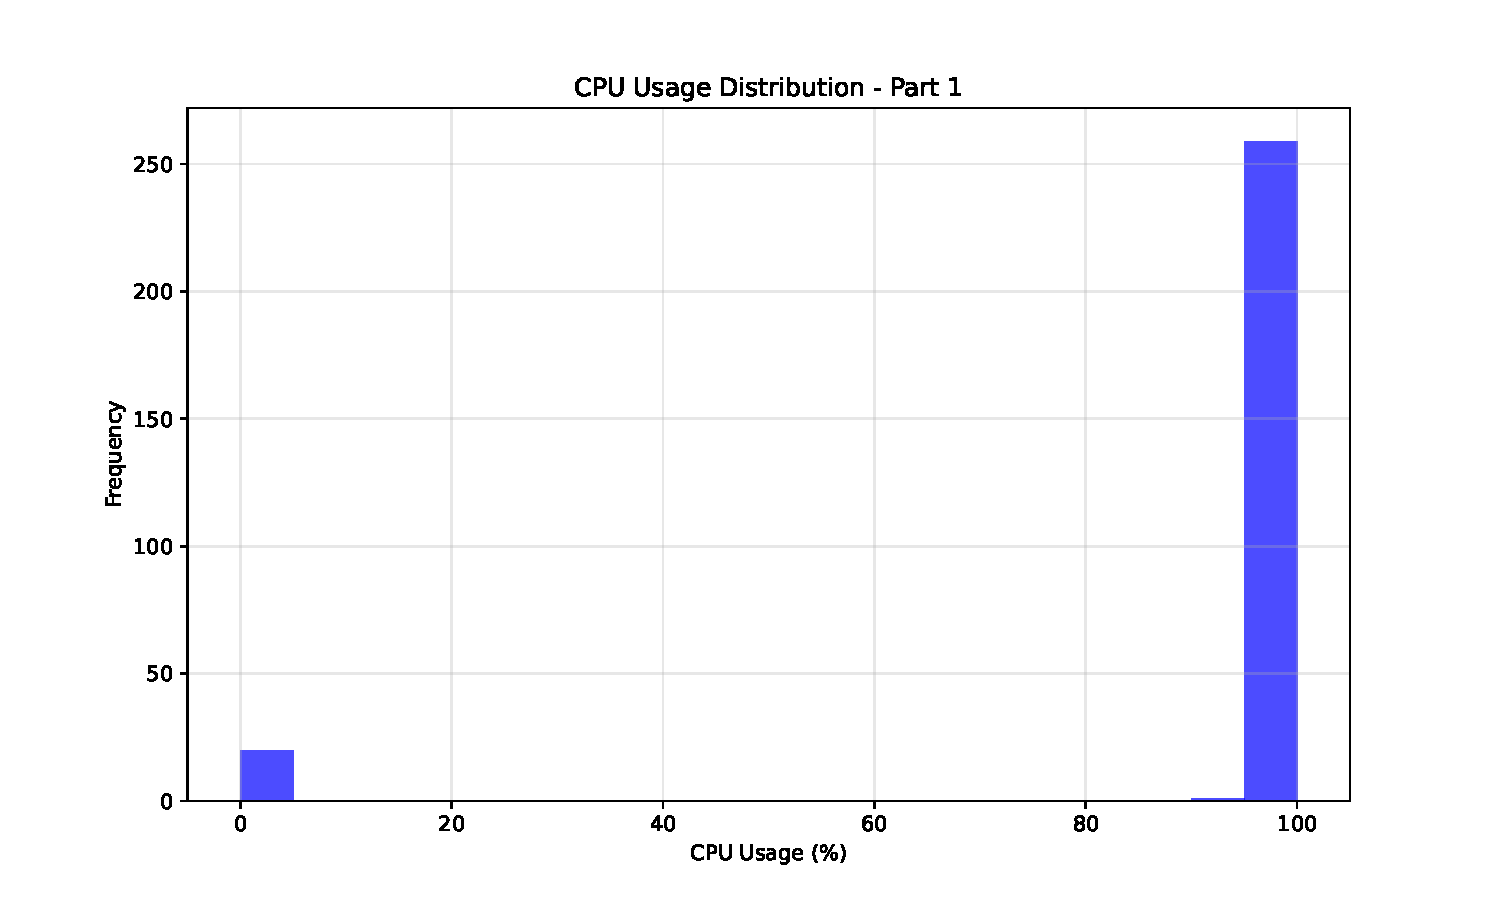
\includegraphics[width=0.8\textwidth]{figures/cpu_dist_part1.pdf}
    \caption{Distribuição do uso de CPU para N processos em N núcleos}
    \label{fig:part1_cpu}
\end{figure}

\subsection{Parte 2: Sobrecarga com N+1 Processos}

Ao executar N+1 processos intensivos em CPU em N núcleos, observamos que o escalonador distribuiu o tempo de CPU quase igualmente entre todos os processos, mas cada processo recebeu um pouco menos de 100\% de um núcleo de CPU. Esse comportamento demonstra o princípio de equidade do CFS: em vez de dar a N processos 100\% e deixar um processo sem recursos, ele reduz a alocação para todos os processos para manter a equidade.

O uso da CPU por processo foi aproximadamente $\frac{N \times 100\%}{N+1}$, o que significa que cada processo recebeu aproximadamente 85-90\% de um núcleo de CPU em um sistema de 6 núcleos. Os estados dos processos permaneceram "R+" durante todo o experimento, indicando que todos os processos estavam ativamente executando, mas compartilhando o tempo de CPU.

\begin{figure}[H]
    \centering
    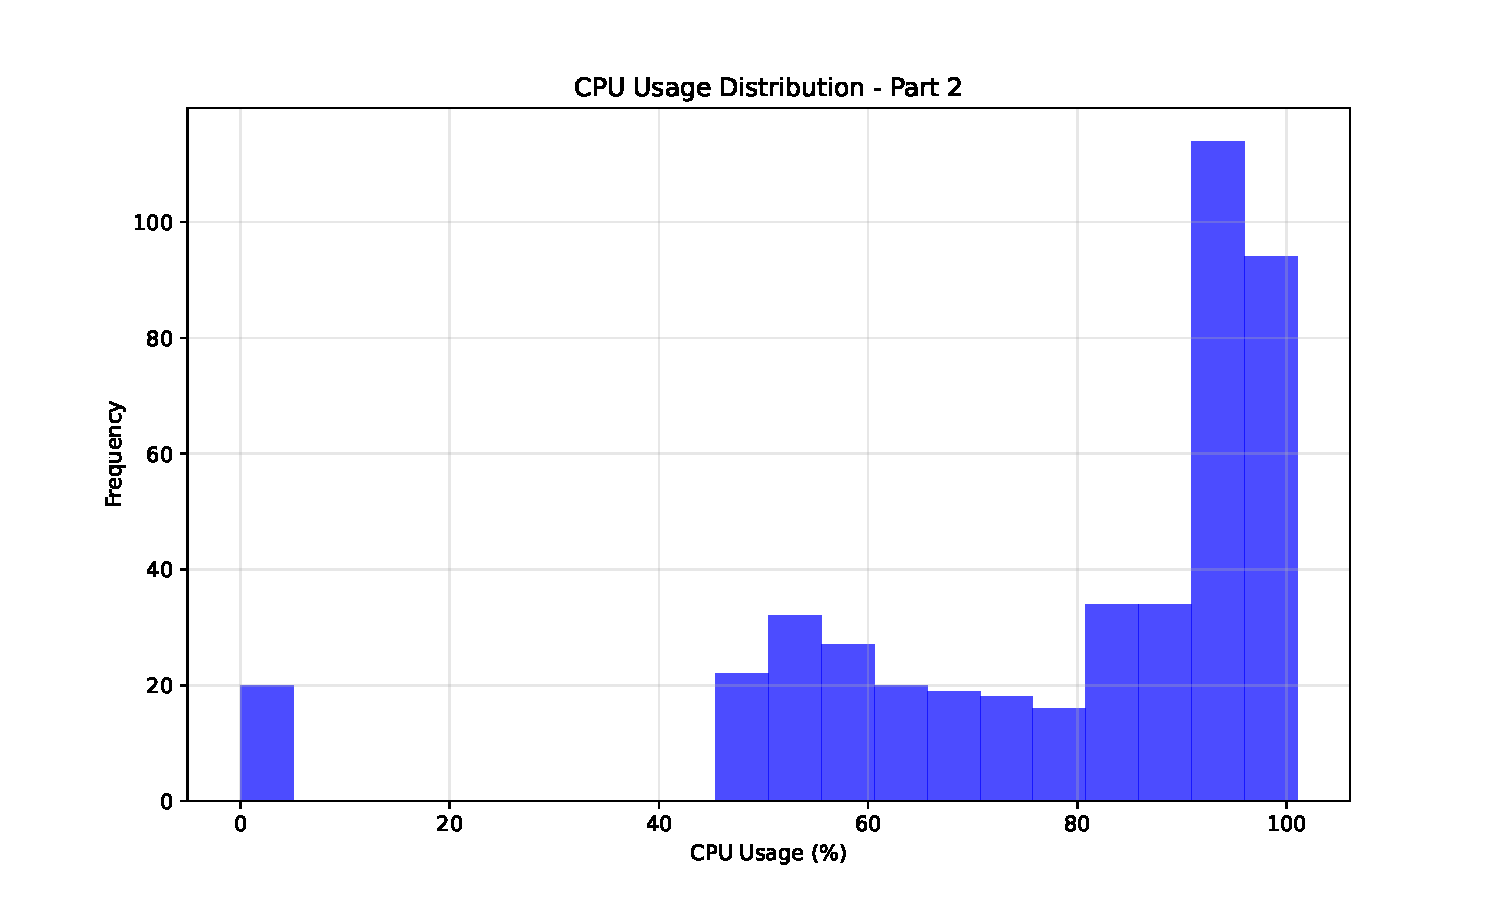
\includegraphics[width=0.8\textwidth]{figures/cpu_dist_part2.pdf}
    \caption{Distribuição do uso de CPU para N+1 processos em N núcleos}
    \label{fig:part2_cpu}
\end{figure}

\subsection{Parte 3: Efeito da Prioridade}

Quando um processo recebeu uma prioridade mais alta usando \texttt{renice -n -10}, observamos que este processo recebeu mais tempo de CPU em comparação com outros processos. O processo de maior prioridade consistentemente mostrou porcentagens mais altas de uso de CPU, demonstrando que o CFS respeita as prioridades dos processos ao alocar tempo de CPU.

O valor nice influencia o cálculo de "peso" no CFS, que determina quanto tempo de CPU um processo recebe. Processos com valores nice mais baixos (prioridade mais alta) recebem mais peso e consequentemente mais tempo de CPU. No entanto, é importante notar que o CFS ainda garante que os processos de menor prioridade recebam algum tempo de CPU, em vez de serem completamente preteridos.
\subsection{Parte 4: Processo Bloqueado por Entrada}

Ao executar N processos intensivos em CPU e um processo bloqueado aguardando entrada, observamos que o processo bloqueado passou a maior parte do tempo no estado "S+" (sono interruptível em primeiro plano). Enquanto neste estado, o processo consumiu recursos de CPU insignificantes.

Quando o processo bloqueado recebeu entrada, ele transitou brevemente para o estado "R+", consumiu algum tempo de CPU para processar a entrada, e então retornou ao estado "S+" enquanto aguardava mais entrada. Esse comportamento demonstra como o CFS lida eficientemente com processos vinculados a E/S, permitindo que eles respondam prontamente a eventos de E/S sem desperdiçar ciclos de CPU enquanto aguardam.

\section{Análise Comparativa}

\subsection{CFS vs. Outros Algoritmos de Escalonamento}

O Escalonador Completamente Justo do Linux mostra várias características distintas em comparação com algoritmos de escalonamento tradicionais:

\begin{table}[H]
\centering
\begin{tabular}{|p{2.5cm}|p{11cm}|}
\hline
\textbf{Escalonador} & \textbf{Características} \\
\hline
CFS & Rastreia o tempo de execução virtual para cada processo para garantir equidade. Processos com menor tempo de execução virtual são escalonados em seguida. Emprega enfileiramento justo ponderado baseado na prioridade do processo. Usa uma árvore rubro-negra para seleção eficiente de processos. \\
\hline
FIFO & Processos executam na ordem em que chegam até completarem. Sem preempção exceto para processos de maior prioridade. Pode levar ao efeito comboio, onde processos curtos esperam atrás de processos longos. \\
\hline
Round Robin & Aloca um quantum de tempo fixo para cada processo em uma fila circular. Garante que cada processo receba tempo de CPU, mas pode levar a alta sobrecarga de troca de contexto. \\
\hline
SJF & Prioriza processos com menor tempo de execução. Ótimo para minimizar o tempo médio de espera, mas requer conhecimento prévio do tempo de execução do processo. Pode levar à inanição de processos longos. \\
\hline
\end{tabular}
\caption{Comparação de algoritmos de escalonamento}
\label{tab:scheduler_comparison}
\end{table}

\subsection{Análise da Distribuição de CPU}

Nossos experimentos revelaram as seguintes observações-chave sobre como o CFS distribui o tempo de CPU:

\begin{enumerate}
    \item \textbf{Recursos Iguais}: Quando os recursos são suficientes (N processos em N núcleos), o CFS aloca um núcleo para cada processo.

    \item \textbf{Contenção de Recursos}: Quando os recursos são insuficientes (N+1 processos em N núcleos), o CFS reduz a alocação para todos os processos em vez de deixar algum processo sem recursos.

    \item \textbf{Influência da Prioridade}: As prioridades dos processos (valores nice) influenciam a distribuição do tempo de CPU, com processos de maior prioridade recebendo mais tempo.

    \item \textbf{Consciência do Tipo de Processo}: Processos vinculados a E/S são tratados de forma diferente dos processos vinculados à CPU, recebendo pronto serviço quando precisam de tempo de CPU, mas não consumindo recursos enquanto aguardam.
\end{enumerate}

\section{Conclusão}

O Escalonador Completamente Justo do Linux faz jus ao seu nome, fornecendo alocação justa de tempo de CPU entre processos concorrentes. Nossos experimentos demonstraram vários aspectos-chave do comportamento do CFS:

\begin{enumerate}
    \item O CFS distribui eficientemente os recursos de CPU quando o número de processos iguala o número de núcleos de CPU.

    \item Quando os processos excedem os núcleos disponíveis, o CFS mantém a equidade reduzindo a alocação para todos os processos em vez de deixar alguns sem recursos.

    \item As prioridades dos processos influenciam a alocação de CPU, mas o CFS garante que até mesmo processos de baixa prioridade recebam algum tempo de CPU.

    \item O CFS lida efetivamente com as diferentes necessidades dos processos vinculados à CPU e à E/S.
\end{enumerate}

Essas características tornam o CFS bem adequado para ambientes de computação de uso geral onde equidade, capacidade de resposta e utilização eficiente de recursos são importantes. Em comparação com algoritmos tradicionais como FIFO, Round Robin ou Shortest Job First, o CFS oferece uma abordagem equilibrada que lida com cargas de trabalho diversas mantendo a equidade.

Os mecanismos de rastreamento de tempo de execução virtual e enfileiramento justo ponderado do CFS proporcionam melhor capacidade de resposta geral do sistema do que algoritmos mais simples, particularmente em cenários de carga de trabalho mista com processos tanto intensivos em CPU quanto interativos.

\appendix
\section{Implementação do Código}

Os experimentos foram implementados usando código C que criou processos e monitorou seu comportamento. A implementação utilizou chamadas de sistema como \texttt{fork()}, \texttt{exec()}, e monitoramento de processos via comando \texttt{ps}.

Componentes-chave da implementação incluíram:

\begin{itemize}
    \item Criação de processos usando \texttt{fork()} e funções de tarefa personalizadas
    \item Monitoramento de processos usando o comando \texttt{ps} redirecionado para arquivos de log
    \item Ajuste de prioridade de processos usando o comando \texttt{renice}
    \item Simulação de processo vinculado a E/S usando uma operação de leitura bloqueante
\end{itemize}

\section{Metodologia de Análise}

A análise foi realizada usando scripts Python que analisaram os arquivos de log gerados durante os experimentos. A análise concentrou-se em:

\begin{itemize}
    \item Estatísticas de uso da CPU (média, mediana, desvio padrão)
    \item Distribuições de estado dos processos
    \item Correlação entre prioridades dos processos e alocação de CPU
\end{itemize}

Métodos estatísticos foram utilizados para analisar os dados e gerar visualizações que destacam os comportamentos-chave do escalonador Linux sob diferentes condições.

\end{document}
